\documentclass[
	fontsize=10pt, % Base font size
	twoside=false, % Use different layouts for even and odd pages (in particular, if twoside=true, the margin column will be always on the outside)
	%open=any, % If twoside=true, uncomment this to force new chapters to start on any page, not only on right (odd) pages
	%chapterprefix=true, % Uncomment to use the word "Chapter" before chapter numbers everywhere they appear
	%chapterentrydots=true, % Uncomment to output dots from the chapter name to the page number in the table of contents
	numbers=noenddot, % Comment to output dots after chapter numbers; the most common values for this option are: enddot, noenddot and auto (see the KOMAScript documentation for an in-depth explanation)
	%draft=true, % If uncommented, rulers will be added in the header and footer
	%overfullrule=true, % If uncommented, overly long lines will be marked by a black box; useful for correcting spacing problems
]{kaobook}
\usepackage[english]{babel} % Load characters and hyphenation
\usepackage[english=british]{csquotes} % English quotes
\usepackage{blindtext}
\usepackage{styles/kaobiblio}
\addbibresource{main.bib} % Bibliography file
\usepackage{styles/mdftheorems}
\graphicspath{{examples/documentation/images/}{images/}} % Paths in which to look for images
\makeindex[columns=3, title=Alphabetical Index, intoc] % Make LaTeX produce the files required to compile the index
\makeglossaries % Make LaTeX produce the files required to compile the glossary
\makenomenclature % Make LaTeX produce the files required to compile the nomenclature
\begin{document}
\title[The Project Documentation Management]{The Project Documentation Management}
\subtitle{Methods and best pratice for a structured redaction and reuse of the project documentation}
\author[Luc Dumont]{Luc Dumont \thanks{A \LaTeX\ beginer}}
\date{\today}
\publishers{Naept Editions}
\frontmatter % Denotes the start of the pre-document content, uses roman numerals

%----------------------------------------------------------------------------------------
%	MAIN BODY
%----------------------------------------------------------------------------------------

\mainmatter % Denotes the start of the main document content, resets page numbering and uses arabic numbers
\setchapterstyle{kao} % Choose the default chapter heading style

% \setchapterpreamble[u]{\margintoc}
\chapter{Why writing project documentation is boring?}

“We’ll have to do documentation again ? Really !”

We hear this a lot when we tell a teammate he will have to write some documentation for the project. We are engineers and we have had to deliver many many documents. So let’s be honest, documentation is boring. But when it is well done, it is a very valuable asset. It allows to make once mind, settle the project, detail, save, index and share ideas and innovative solutions (God bless Ctrl+F). Documentation would be so much less painful if it wasn’t for some productivity traps that are so time consuming and generate pressure. Fortunately they can be avoided …

Here is a non exhaustive list of what is unpleasant when writing a document, and how to overcome it.

\section{Writing about a topic we do not master}
There is often only one person dedicated to write all the documentation of a project. It avoids to manage a planing for several editors. Besides the final product will have one consistent tone. But this one person may not master all the different fields of technology taking part in the project to give a complete description of them. This situation has been encountered by a person we met.

\begin{kaobox}[frametitle=A former teammate engineer destimonial]
	I had been asked to write the tests to do on a product to ensure it meets our customer needs. It was a complex task because I was completely unfamiliar with one of the involved technologies. I had to ask to the expert and I worked hard to understand how it was working to finally write some relevant tests. It took me several iterations of them but it ended up working. I up skilled a lot on this technology but we may had lost some time and I got some cold sweats.
\end{kaobox}

Giving someone a task he isn’t skilled enough to perform without some learning can lead to an unsecured mindset. But sometimes, by lack of available experts, we cannot do otherwise.

Today there are more and more collaborative softwares easing the teamwork (you can share a document and comment it in real time with Microsoft Word or Google Docs for example). We have met lots of companies making their own tutorial videos to share some specific knowledge between collaborators. Besides, the “reuse”, which means starting from previous documents to write the new ones, is becoming the rule. It is always easier to update a previous revision and adapt it to the new project, than starting the document from scratch.

\section{The WYSIWYG editors}
WYSIWYG stands for: “What You See Is What You Get”. It means what you see on screen is its real rendering. This is how works the main text editors like Microsoft Word. This makes those softwares very intuitive and easy to use. Everybody knows how to write something on Word!

But when you write project documentation, you probably need to add comments, track modifications, draw tables, put some automatic fields (page numbers, etc)...

This leads the software to use lots of RAM to be able to render the final view of your document in real time with all those features. It does it seamlessly for a short file. But your computer might start to sweat when your document reaches the hundred of pages. Then the text editor reactivity is getting slower and can finally crash (true story)!

\LaTeX{}

To avoid hitting the save button every minutes, there are text editors with different philosophy. LaTeX is one of those and it is free. But it requires some learning first. Its way to do is to differentiate the content from the document layout in different files. On one side you write your text with tags in it. Those tags will indicate where you want the graphical features such as a figure, a table, a title, etc. On the other side. At this moment your text doesn't look like the final rendering at all ! On a second file you configure the display of those graphical features. Finally you run LaTeX on those files and it builds your document. You may have to run several times LaTeX with different settings to get the exact document you had in mind. But then you will never have to correct the layout. It will never change because of a text modification. Content and layout do not interfere.

Ok, I confess it seams a little more touchy than Word. But you should give it a try because it is so much more powerful and rather easy to master !
Fortunately the WYSIWYG text editors get auto-save feature that are more and more effective.


\section{Validation workflows}
Usually every document shall be delivered to the customer. To ensure the document reaches the quality standard of the company, it must be checked by several reviewers through a validation workflow.

But the reviewers expectations may vary if they don’t know the project with the same level of details. So a simple document review can turn into an argumentation about the project itself. Here we go again, those reviews must be planed:

\begin{enumerate}
	\item Select reviewers for the project and stick with them all along. You can assign them to specific parts of the document corresponding to there expertise.
	\item Schedule the reviews in a finite period of time.
	\item Collect their remarks in one place, like a spreadsheet for example. This will ease their management en then the document update.
\end{enumerate}


\section{The level of detail}
Whatever the product, its specifications can be two pages long or one hundred. The difference lays in the level of details.

There is no miracle spec. They can be very light, it is cheap but you risk to put the project on hold with non-anticipated issues. They can be very detailed and plan everything but not only they are very expensive but every review will be very long.

So you have to meet halfway. A good practice is to make a first iteration allowing someone who doesn’t know the project to understand it and start working on it. Then, very regularly, with small steps, update the document throughout the project. Be careful not to overkill the quality, it is not a piece of art, it is a tool. Documentation must not drain you effort over more critical activities.


\section{The lack of interest}
Some documents have no other purpose than being archived. They are just new entries to some dead database and will never be referred back to ever again. They are artifacts from an obsolete but persistent workflow. The french philosopher Julia de Funes says that loss of meaning happens when the purpose disappears in favor of its mean.

It is time to question this workflow because those documents have a cost (an not only a financial cost). What impact on the collaborator mindset will have this lack of interest for his work?

On the other hand, such a documentation can be highly valuable! It can be a precious asset to kickstart similar new projects. If they are just saved and correctly indexed in a database (like Sharepoint), a simple request on its search engine will rapidly identify the most relevant documentation to reuse. And by constantly updating this database, the company not only saves but grows its knowledge, its expertise. It turns this previously frozen load into a living strategic asset. The author becomes aware that he is building knowledge other will trust and use. It is a far more gratifying activity!

\section{Working blind}
The blank page syndrome is not a novelist privilege. Being in charge of a complex specification document can be petrifying if we don’t know where to start. Should I start by this element or this one ? Haven’t I forgot anything ? Is it precise enough ? It is really clear ? Should I explain this or is it obvious?

It is always a good move to start from something known and verified. We take a previous document, we drop what is out of context, we keep the frame and what is reusable and we start from here. The old parts will help us, guide us to be more exhaustive about the new project.

The next step is to build templates with pre-filled sections. It avoids us to rewrite over and over the same elements in all documents. Those templates can have entitled sections for every possible aspect of the projects. All of them will rarely be filled but they help ensure we forgot nothing. Project after project, those templates are updated and the document quality rises up.

The website FYI presents a very large amount of templates and dashboards for every productivity tools to Getting Work Done! (their moto)

\section{Conclusion}
After all, we see that documentation might not be a problem at all. Organization, effective management and methodology can easily turn what was a painful activity into a real engine for productivity and motivation!


% \setchapterpreamble[u]{\margintoc}
\chapter{Why writing documentation is boring}
\label{sec:WhyBoring}

Writing a specification document can feel ea“We’ll have to do documentation again ? Really !”

If only that could be so easy. Sometimes it is. But usually not. We will go through 4 major difficulties in this process from a simple McDonald’s order to a wedding planning! 

12:15 AM in a McDonald’s fast-food:\\
– Hello, I’d like a Big Mac, a Coke and a large portion of fries please.\\
2 minutes later :\\
– Here is your order, have a nice day.\\
– Thank you, goodbye.

8:30 PM in a fancy restaurant:\\
– Honey, will you marry me ?– Yes !!!\\
One year later, 2 weeks before wedding:\\
– Great Scott! Nothing is going well! The whole table disposition from the wedding planer has to be remade : Anthony cannot bear his brother and my cousins have canceled. All the tablecloths are taupe but they should be beige. We totally forgot to organize the brunch. And you remember your Mexican music band? Wee cannot afford it!!!

\begin{kaobox}[frametitle=Disclaimer]
	This article isn’t in any way a celebration of the well-know fast food license. But it is a very good example of how a customer experience can be fully optimized
\end{kaobox}

Either for a project as quick as a fast food order, or for one as ambitious asa wedding planning, the first step is always the same. We list all that we want and give it to some professionals who will take care of everything.In both cases, we identified 4 characteristics that are very important to master if we want the most seamless communication possible. Let’s dive into them.


\section{The context}

In the McDonald’s order placement scenario, the context issue is solved by your presence into the restaurant. If, by any odd circumstance, you would order a burger in a shoe shop for example you would get a good laugh from the seller or maybe a suspicious look.

In the wedding case, we observe that we haven’t explain enough of the family situation to the wedding planer: the enemies brothers and the not so reliable cousins.

It is very important to give the most complete context for a project to our supplier, to detail our activity. Like that, even before entering the core of your need, he will be able to tell if he is qualified enough for the job or not. To do so, you can present:

\begin{itemize}
	\item Your company, its activities, some technical concepts you need your supplier to understand
	\item Your market and your customers
	\item The project your need is about
\end{itemize}


\section{The vocabulary}
At McDonald’s, the vocabulary to order a menu is clearly defined thanks to the panels above the cashiers. They show all the burgers and side dishes available. Their combinations are rather finite and the customers have all the time to build their order while they wait in line.

For wedding, we can have very precise expectations, like beige tablecloths for example. But if we haven’t correctly defined with the planer what we have in mind when we talk about the beige color, we can end up with taupe!

So clearly stating the vocabulary is essential. There is a probability that you will employ the same wording but with a slightly different meaning. That difference can generate big consequences on the budget or the planning by the end of the project before you understand why.

A simple glossary of the most important elements, placed in the opening of the document, can ensure all the stakeholders that they speak the same language. Do not hesitate to update it during the project in any doubt appears.


\section{The maturity}
This is the most common characteristic in the fast food orders: how many customer arrive at the cashier and are still building up their order. But it’s in the name: fast food! If the order isn’t complete, it won’t take the customer too much time to come back with a new order.

Maybe the Mexican band wasn’t necessary for an already beautiful wedding. Or at least, it wasn’t totally affordable. It would probably be wiser to abandon this “requirement” to secure the event.

More seriously, it is difficult to precisely estimate the maturity of a project at the beginning. Is this item relevant? Useful? Is it a “must have” or a “nice to have”? Do we really need a hammer to kill a fly? Or a rolled newspaper is enough? We can employ the 5 why technique: questioning a need 5 times in a row to find out its root, its prime cause.
We can also openly talk about it with our supplier and give him the opportunity to make suggestions, and for us to trust its expertise.


\section{The exhaustiveness}
We are always asked if we want anything more in a fast food. It is to drive us to buy more? It is to be sure we, the customers, are always pleased? I will leave you to this mystery. But this question has the benefit to ensure an higher maturity, completeness of our order, avoiding us to come back for something we would have forgotten.

Oh, oh, oh! We totally forgot to think about the brunch for the day after! We need a whole new budget for it and talk about it with the caterer! This wedding planner is very lame. He should have warned us.

This issue goes hand to hand with the maturity of our needs. Exhaustiveness asks us “Did you think of it all? Have you not forgot something?” Very hard to tell in advance.
To secure those risks and avoid any “holes in the racket” (we say “trou dans la raquette” when something is missing), we can check what we did in previous projects. We can consult their documentation and use it like a starting checklist. Some parts could be completely reusable and some other may need minor updates. In the same mindset, we can build templates for the projects: pre-filled documents with commonly used chapters and checklists. Some will be abandoned, some will be kept, augmented, optimized

Once again, we can brainstorm with our supplier and summon his expertise. His fresh look upon the project can enlighten some dark areas.

% \setchapterpreamble[u]{\margintoc}
\chapter{Needs assessment : some good practices}
\label{sec:NeedAssessement}
When we write a needs assessment or a specification document for a supplier, we try to be as complete as possible. The document turns into a list of expected features. Here are some good practices to build the most efficient request.

\section{Sorting the requirements by themes}
The more requirement we have, the more difficult it will be to get the big picture. So we have to sort them by their subject, by the technology they are about, or by the expertise they require.

For example, to specify a bike, we gather as follow:
\begin{itemize}
    \item All the requirements about the wheels
    \item All the requirements about the brake system
    \item All the requirements about the gear management
    \item \dots
\end{itemize}

Therefore the supplier will easily be able to choose his best qualified experts for the job. The needs assessment document can now be shared with all of them, and each of them can take on the part about his field of expertise.

\section{The shorter, the better}
When writing a needs assessment, we may intend to write long descriptions for several reasons:

\begin{itemize}
    \item we are in a train of thoughts
    \item we describe several connected elements
    \item the subject is complex and requires lots of details
\end{itemize}

But the problem happens when the customer brings an evolution to its initial assessment. We have to find out what are the impacts on our features specifications. Without an accurate indexing of the requirement and a clear view of their content, we will have to read the whole document again. That can take a lot of time.

But if, from the beginning, we have tried to write the shortest possible requirements, each of them deals only with a specific point, it will increase their quantity but it will also strongly optimizes the following:

Their \textbf{indexing}: one requirement describes one limited subject.

The easiness of their \textbf{update}: we know at one glance if the requirement must be updated because of an evolution.

Their \textbf{traceability}: it is way easier to link the need to the feature.

Their \textbf{testing}: the shorter the requirement, the easier to prove that the final product matches it.

Their \textbf{reusability}: in a future project, if the client defines a similar need, it will be very easy to reuse the requirements from a previous project. You may have to perform some adaptations but they will be limited. Just like a piece of Lego you can reuse in a new construction.

\section{A needs assessment requirement must describe a need, not a feature}
When we write a needs assessment, the purpose is to subcontract the product development to a supplier. We do so because we do not have the resources or the knowledge to do it ourselves.

But if we have a very detailed idea of what we want, we may be tempted to write a full feature specification. Which is a totally different document and we advise you to agree with your supplier about it. Unless, be careful not to give too much specific details and force your supplier. By giving him to much technical details, you won’t summon the expertise you were asking in the first place by hiring him. It is risky for the project to mix your need and the solution specification in the same document :

\begin{itemize}
    \item Are you sure the features you have in mind will match your needs? (Have you ever heard about the XY problem?)
    \item Your feature solutions, are they all compliant?
    \item What are you expecting from your supplier? An expertise or just some manpower?
    \item What about its added value?
    \item What about its responsibility?
\end{itemize}

That’s why it is important to distinguish your needs from the final product features.

\section{Using "shall"}
English language is very generous on how to express what we want. Some of the manners can be ambiguous and may compromise the message we want to deliver.

\begin{itemize}
    \item “I would like“, “I wish“… Is this a strong order or the expression of a nice to have?
    \item “I want“… Is it a personal request? Is it part of the contract?
    \item “It has not to”… Should we understand it has a strong prohibition or the freedom not to do it ?
\end{itemize}

First of all, you can choose any verb but the most important is to choose one and stick to it during all the project. A commonly used one we recommend is to employ “shall”. It is simple, kind of binary and rather not questionable:

\begin{itemize}
    \item “XXX shall be…” or “XXX shall do…“: it describes what is expected
    \item “XXX shall not be…” or “XXX shall not do…“: it describes what must not be expected
\end{itemize}

\section{Pay attention to all the possible interpretations}
A same text can be understood differently depending on the reader’s expertise, experience, position and even his current state of mind. So there is a chance that he has a slightly different interpretation than yours. This risk must be considered seriously as it can lead to severe project shift. Do your words express your thoughts? Is there any room for a misunderstanding? Do you share with your supplier the same meaning for every concepts of the project? The road to hell is paved with good intentions.

So, before delivering a document, a simple peer review by one of your teammates will very efficiently reduce the risks of misunderstanding. And adding a glossary at the beginning of the document to define the sharpest concepts will reduce the risks even more.


\section{Is your need testable?}
Is it even possible to check that the product matches every specific requirement?

Imagine that one of your requests asks for “the fastest” car. Alright. How can your supplier ensure you that the car he delivered is “the fastest”? This is a tricky demand hardly verifiable. First of all, how fast can a car go today? What if this speed is different than the one you had in mind? Who is right?

It is much safer to build the requests with measurable elements. These won’t let any doubt about what you are expecting and will be undeniably verifiable.

“The car shall be able to reach the speed of 250 kph”. The delivered car goes up to 300 kph. Ok! It matches the need, the requirement is validated!

For more details about tests, read our article about validation plans. It is also in french, we will publish it in english soon too.


% \setchapterpreamble[u]{\margintoc}
\chapter{Reading sheet, an easy tool for collaborative review}
\label{sec:ReadingSheet}

Finally ! You did it ! The document is finished. But before definitely freeze it, it has to be validated. So you send it to several people who will read it and comment it. But one week later, you have dozens of e-mail from them and 4 different corrected copies of your document. Those exchanges have brought more questions than answers. The reading sheet allows you to structure the validation process and to take every remark into account.

Depending on the size and complexity of the project, it is required to validate its documentation by one or several people:

\begin{itemize}
    \item The project manager who is responsible for the customer
    \item A peer reviewer who checks the technical content
    \item A quality expert who ensures the document matches the company’s quality criteria
    \item …
\end{itemize}

The customer who tells if the document meets his needs.
Without a clear workflow, every reviewer can comment the document in a different way:
\begin{itemize}
    \item by mail
    \item by telling you his remarks at the coffee machine
    \item within his own document copy
    \item in the MS Word comment section
    \item by hand-writing his remarks on a print
    \item …
\end{itemize}

Managing so many different channels can jeopardize the final quality of the document. How to be sure none of the remarks is lost? Is there some duplicated ones? Are they all consistent? Etc.

\section{One file to collect them all}
The reading sheet is a tool to collect all the remarks about a document (or anything else) in the same place and organize them to address them all.

This is a simple spreadsheet, an MS Excel file, in which every line is a reviewer remark. It contains several columns to fill. Those columns are indicators allowing to sort the remarks and ease their management. In the following paragraph we will detail the most commonly used columns.


\section{The columns}

Here is an example of a reading sheet based on the feedback of our own experiences and the ones of people we met.

\begin{table*}[h]
	\centering
		\begin{tabular}{|c|c|c|c|c|c|c|c|c|c|}
			\hline
			\ ID & Location & Category & Severity & Description & Reviewer & Responsible & Status & Comment & Action \\ 
			\hline
			&&&&&&&&&\\
		\end{tabular}
	\caption{Headers for a reading sheet}
	\label{tab:HeaderRS}
\end{table*}

This list isn’t exhaustive. Some of them might be useless and you might need some other depending of your process. Please share with us in the comment section those data you use in your own reading sheets.

\subsection{ID}
It is a simple but unique number, incremented for each remark. The purpose is to identify it. If a remark must be erased, its ID has to be erased too and it cannot be used for another one or it could lead to misunderstanding.

\subsection{Location}
Any remark has to be precisely located! The author must not be forced to read the whole document to find the object of the remark. It wouldn’t be very efficient.
A first way of doing this is to locate it with the document page. But it isn’t the best practice because if a section is added to the document, for example, the updated can turn to be totally irrelevent.
The ideal way is to locate the remark with the smallest paragraph title its object belongs too. Like this, it doesn’t matter if the paging changes. The author will quickly find it with the table of content.

The location shall be given by the reviewer.

\subsection{Category}
All the remarks are not from the same kind. They can be about:

\begin{itemize}
    \item a comprehension question
    \item a spelling mistake
    \item an author misunderstanding of the need
    \item etc.
\end{itemize}

Therefore remarks can be sorted by categories. It will be easier to manage them. Fro example, the author may want to fix all misspelling ones before going to the semantics.

It is important to have a limited number of categories for the sorting to be useful. But on the other hand, it is required that list to be exhaustive enough to cover any kind of remarks. Here are some possible categories:

\begin{itemize}
    \item Question
    \item Misspelling
    \item Nonsense
    \item Layout
    \item Error
\end{itemize} 
Category shall be given by the reviewer.

\subsection{Severity}
Severity is a second sorting criteria. Two remarks from the same category can have different weight. This weight can be defined by the severity.

For example, the severity scale can go from level 1 telling the remark is painless for the project, to level 5 telling the pursuit of the project is stopped as long as this remark isn’t solved.

It is really important that this severity scale is clearly defined and shared with everyone before starting the reviews.

Severity shall be given by the reviewer.

\subsection{Description}
This is the description of the remark itself. It is important this description is as detailed as possible. You can insert a short document extract to ease its understanding, highlight important words. It shall be precise enough for the author to not have any doubt about the issue.

Description shall be given by the reviewer (obviously).

\subsection{Reviewer}
If the author knows who gave each remark (several reviewer can add remarks to the reading sheet), he will know who to ask if he needs further information to solve the issue.

Reviewer shall be given by… the reviewer.

\subsection{Responsible}
Here we talk about the person in charge of solving the remark. As this person can be different for some remarks (many people may have written the document together), the person responsible must be defined for each remark.

But it is not up to the reviewer to decide who is in charge of his remark, beside he may not have a clue about who is competent for it.
If there is only one author for the document, so it’s a no-brainer: responsible = author.
If there are several authors, there must be a manager driving the team. So it is up to him to tell who is in charge of each remark.

\subsection{Status}
It simply is the status of the remark. Depending on your review workflow, this status can take several values. Here are some examples of possible values:

\begin{itemize}
    \item \textbf{Open} (set by the reviewer)\\When a new remark is added, it is “open” for resolution, meaning it shall be processed by the responsible.
    \item \textbf{Duplicated} (set by the person responsible)\\If by any chance a remark tells the same thing than another one, the responsible gives this status to it. It happens when several reviewers use the shame reading sheet to gather their remarks.
    \item \textbf{Accepted} (set by the person responsible)\\It is a temporary status. On a first hand, the responsible may have a look on all remarks at once. He may want to check for the duplicated ones or to see if all of them are relevant. When he wants to tell if a remark is relevant and he is willing the solve it, he sets this status.
    \item \textbf{Rejected} (set by the person responsible)\\But when he believes a remark is not relevant, he can set it to”Rejected”. He shall explain why it is irrelevant in the comment section. Then the reviewer will decide if he agrees.
    \item \textbf{Corrected} (set by the person responsible)\\The responsible has accepted and fixed the document according to the remark. He tells it is “Corrected” then the reviewer can check if he is OK the correction.
    \item \textbf{Closed} (set by the reviewer)\\If the correction is satisfying, the reviewer can set the remark to “Closed”. Case closed!
\end{itemize}

\subsection{Comment}
This section can be used by the responsible to bring a comment on the remark resolution. He can explain here how he corrected it.
This is where he shall explain why he eventually rejected the remark.
If the remark consisted in a simple question, this is where the answer shall be brought.

Be careful to not turn this comment section into a chatroom about the remark.

If required, the comment can be added by any stakeholder.

\subsection{Action}
Some remarks and resolutions can have a higher scope than just updating the document. They may require to update the whole project, change the contract, the planning, the budget, the product…

So one remark can have some ripple effect implying the use of a project dashboard action, a bugtracking issue (see our french article, but soon translated)… Those item have their own identification references. So you can use the Action column to quote those references and ensure the traceability of the cross-application resolution.

If required, the action shall be given by the responsible.

\section{Best practices}
\subsection{Index the reading sheet}
As soon as you create a new reading sheet, give it a unique reference. It will allow everyone to quote it in the document it talks about and ease their management if you have several of them.
\subsection{Use one for each document delivery}
Every time you send a document to someone, if this someone can comment it, join a blank reading sheet. So he can add its remarks directly into it, saving you the task to copy and past them from his e-mail.
\subsection{Traceability}
When you start to update a document with all your reviewers remarks, indicate in the document that it has evolved thanks to the reading sheet <insert its reference>. So anyone can track back the origin of those evolutions.
\subsection{Precision}
Never hesitate to give the most exhaustive description for a remark. The responsible shall have enough information to not need to call you back to remove a doubt.

Once more, the location in the document of the object of the remark shall be as precise as possible for the responsible shall not lose time finding it.

\section{Pros and cons}
\subsection{Pros}
You can build a reading sheet out of any spreadsheet editor (MS Excel, Google Docs, OpenOffice…). So that is a really easy tool available to anyone.

It is not only applicable to a document review but, actually, to any kind of reviews: source code, graphic elements, product… As soon as you need to collect remarks, the reading sheet is relevant.

Even if there are several reviewers, you can send them each a reading sheet and then gather all of them into one (you can even write a script to do it automatically). But with the today online editors, it is even easier to work on a shared document.
\subsection{Cons}
Be careful not to use a reading sheet and its comment section as a forum with an endless message chain. Comments shall just be comments. Otherwise just pick up the phone.

Obviously it is another file to manage in the project and you may already have lots of them.

You better have a big screen or even two. It is nice to have the document you are reviewing on a side and its reading sheet on the other side. Switching from one to the other on a single screen might drive you crazy.

\section{Conclusion}
The reading sheet is a very easy and versatile collaborative tool. It allows you to structure and easily manage any reviewing process. Even if more and more software come with comment features, a reading sheet is a quick and simple solution to implement with anyone regardless of having the last fancy webapp. You can find a reading sheet template for free on our Github repository.

% \setchapterpreamble[u]{\margintoc}
\chapter{The traceability matrices}
\label{sec:TraceabilityMatrices}

In a customer request for proposal, the need is usually given through a list of requirements. The supplier sends back a proposal showing his solution through a list of specifications. The coverage between requirements and specifications can take different shapes:

\begin{itemize}
    \item 1 to 1: one specification covers one requirement
    \item 1 to many: several specifications are used to cover only one requirement
    \item Many to 1: several requirements are covered by one specification.
\end{itemize}

But in practice, it is rather a mix of the three leading to a maze of coverage. Fortunately the traceability matrix shows up to bring some order.


\section{Traceability, this entangled mess}
A document size can vary a lot depending on the different fields of activity it deals with. To explain this, I will take an example I know well. Consider a request for proposal (RFQ) about an aeronautic calculator. Please don’t leave yet! I’ll make it clear.

In a plane, there are dozens of calculators. Those are computers without a screen or a keyboard. They manage everything, from the air conditioning to the brakes, the doors, the electrical power distribution, etc. Whether their tasks are complex or very complex, their request for proposal can easily reach a hundred pages and hundreds of requirements. Several expertises are involved to describe all the requirements. For example:

\begin{itemize}
    \item electronics for the circuit boards
    \item mechanics for the case housing the circuit boards
    \item developers for the embedded firmware of the circuit boards
    \item etc.
\end{itemize}
Then this RFQ is sent to a supplier. He will study it with his teams to build the specifications. Sometimes several requirements can be covered by the same specification.

\subsection{Many to one}
Customer requirement 1: the circuit board shall be hermetically protected\\
Customer requirement 2: the case shall have the following measurements : X, Y, Z

Supplier specification 1: the case shall be from the brand B and the model M

Therefore the supplier specification hits two birds with one stone because the chosen case matches both the requirements.

\begin{figure}[h]
    \centering
    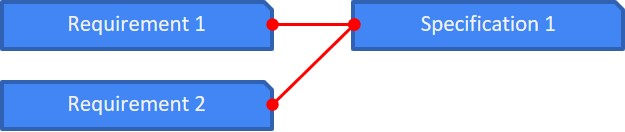
\includegraphics[]{ManyToOne.jpg}
    \caption{2 requirements covered by 1 specification}
    \label{fig:ManyToOne}
\end{figure}

\subsection{One to many}
But sometimes, it is the other way around! The requirement is so complex, it requires several specification to be fully covered:

Customer requirement 3: the circuit board shall be fully operational while the plane is flying (it’d better be).

Supplier specification 2: the electronic components of the circuit board shall be from the S series. The S series components stay operational even at temperatures below -50°C (this is the outdoor temperature at cruising altitude).

Supplier specification 3: the case shall have an S shield to protect the circuit board from electromagnetic fields.

Supplier specification 4: the case shall be mounted on suspending plot to protect the circuit board from mechanical vibrations.
\begin{figure}[h]
    \centering
    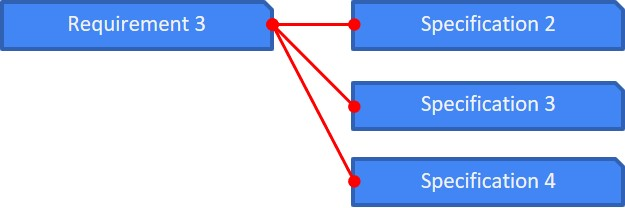
\includegraphics[]{OneToMany.jpg}
    \caption{1 requirement covered by 3 specifications}
    \label{fig:OneToMany}
\end{figure}

So we see here that the complexity of the coverage between requirements and specifications can quickly increase. Just like a spaghetti dish!

\begin{figure}[h]
    \centering
    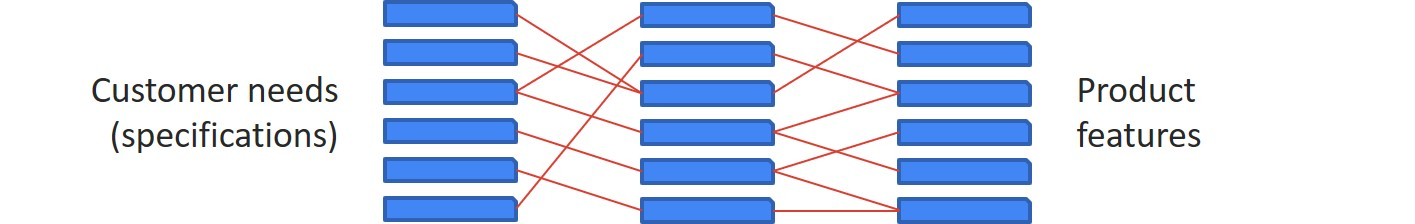
\includegraphics[]{traceability}
    \caption{Many requirements entangled to many specifications}
    \label{fig:WholeTraceability}
\end{figure}

\section{Ok but how exactly?}
\subsection{The structure}
A traceability matrix is an two-columns table where are exhaustively listed every coverage link between every requirements and every specifications. Our previous example would give the following matrix:

\begin{table*}
	\centering
		\begin{tabular}{|c|c|}
			\hline
			Customer Requirements & Supplier Specifications\\
            \hline
            Customer requirement 1 & Supplier specification 1\\
            \hline
            Customer requirement 2 & Supplier specification 1\\
            \hline
            Customer requirement 3 & Supplier specification 2\\
            &Supplier specification3\\
            &Supplier specification 4\\
            \hline
		\end{tabular}
	\caption{Downstream Traceability Matrix}
	\label{tab:DownstreamTraceabilityMatrix}
\end{table*}

On the left, there is the list of the customer’s requirements in the same order they appear in the RFQ. There are given by their title only (or their ID) to avoid an overloaded table.
On the right, for each requirement, the list of the covering customer specifications.

It is very important that on the left column, each requirement appears once and only once. The purpose here is to ensure every requirement is covered by at least one specification.
On the contrary, on the right column, we observe the supplier’s specification 1 is listed twice. This is absolutely normal as this specification matches both customer requirement 1 and customer requirement 2.

\subsection{The point of view and coverage quality}
We can say this matrix adopts the customer’s point of view. It goes from the RFQ to the specifications, that is why it is called the \textbf{Downstream Traceability Matrix}. Once completed, we know exactly the coverage of the customer need. And if one requirement as no specification match, we know the specification document isn’t complete.

But be careful as the devil always hides in the details! The traceability matrix can only tell if a requirement is covered by a specification. I cannot tell if this specification IS ENOUGH to cover the requirement.
Let’s consider again the customer requirement 3. We see it is covered by the following specifications:

\begin{itemize}
    \item Supplier specification 2
    \item Supplier specification 3
    \item Supplier specification 4
\end{itemize}

For example, if the supplier specification 4 is omitted, from the matrix point of view, the customer requirement is still covered. But in reality, without the specification 4, the product wouldn’t match the need.

\section{The other traceability matrices}
We can change the point of view of the matrix to observe the project’s traceability from another angle to ease its management.

\subsection{Upstream Traceability Matrix}
We saw the customer’s point of view with the downstream traceability matrix. Let’s check the supplier’s with the Upstream Traceability Matrix.

\begin{table*}
	\centering
		\begin{tabular}{|c|c|}
			\hline
			Supplier Specifications & Customer Requirements\\
            \hline
            Supplier specification 1 & Customer requirement 1\\
            & Customer requirement 2\\
            \hline
            Supplier specification 2 & Customer requirement 3\\
            \hline
            Supplier specification 3 & Customer requirement 3\\
            \hline
            Supplier specification 4 & Customer requirement 3\\
            \hline
		\end{tabular}
	\caption{Upstream Traceability Matrix}
	\label{tab:UpstreamTraceabilityMatrix}
\end{table*}

On the left, we list the supplier’s specifications in the order they appear in the specification document delivered to the customer, avoiding making duplicates.
On the right, facing each specification, we list all the requirements it covers. This time, it is OK if there are duplicated requirements. It tells that one requirement is covered by several specifications, proving the supplier’s solution is strong and relevant.

This point of view shows if all the specifications cover the requirements and how many requirement are covered by each specification (we will see that sometimes a specification covers nothing)

So in the project’s roadmap, specifications covering the highest number of requirements can be prioritized. In our example, it can be strategic to develop supplier specification 1 to rapidly cover several requirements. Consequently, we can faster reach the minimum valuable product to show the customer. Then we iterate upon it by adding more and more features (aka specifications).

\subsection{Non-covering specification matrix}
It happens that the supplier designs additional specifications covering no requirement. Strange isn’t it?!

Not necessarily. Those orphan specifications may describe constraints for the supplier independent from the customer’s need. But the supplier want to mention them on the specification document to share them with its customer.

For example, the supplier is used to a software, he can tell his customer he will use it through a specification. So that specification will be mandatory without covering any need.
Or the supplier has a special discount for specific components, so he tells thought a specification that he will use this brand over another.
Last example: reading the RFQ, the supplier identifies a hidden need that doesn’t appear in the customer’s requirements. He can add it in his specifications.

He could put those orphan specifications in the upstream matrix, but they would face no requirement. That could bring doubt upon the document: is it a mistake? Is it normal?

To avoid those questioning, the best is to create a new table listing only those non-covering specifications.

% TODO : faire en sorte que le tableau n'apparaisse pas collé au précédent. Une histoire de flottant je crois.
\begin{table*}
	\centering
		\begin{tabular}{|c|}
			\hline
			Non-covering specification matrix\\
            \hline
            Supplier specification 5\\
            \hline
            Supplier specification 6\\
            \hline
            Supplier specification 7\\
            \hline
		\end{tabular}
	\caption{Non-covering Specification Matrix}
	\label{tab:NonCoveringSpecificationMatrix}
\end{table*}

\subsection{Evolution}
It is inevitable! Whether the RFQ or the specification document are intended to evolve. Because the need is more mature, because of the discussions and new ideas come out or bring corrections…

In the document revision 2, some requirements have been updated. But not all of them. So what? Should we read the whole document again? The 200 pages? To only find 3 or 4 modifications?! No! Because there is an evolution matrix!

This matrix doesn’t connect two different documents, it links two revisions of the same document! For example, let’s imagine the RFQ has had 3 modifications as follow:

\begin{table*}
	\centering
		\begin{tabular}{|c|c|}
			\hline
			Evolutions & Comments\\
            \hline
            Customer requirement 2 & Deleted\\
            \hline
            Customer requirement 3.2 & Updated\\
            \hline
            Customer requirement 4 & New\\
            \hline
		\end{tabular}
	\caption{Evolution Matrix}
	\label{tab:EvolutionMatrix}
\end{table*}

\subsection{A deletion}

\begin{table*}
	\centering
		\begin{tabular}{|c|c|}
			\hline
			Evolutions & Comments\\
            \hline
            Customer requirement 2 & Deleted\\
            \hline
		\end{tabular}
	\caption{A deletion}
	\label{tab:Deletion}
\end{table*}

The customer has simply deleted a requirement. It was no longer required or what it described was non longer needed. A deletion in a 200 pages document might be missed. But its impact on the project might be huge because all the specifications that used to cover it are no longer needed either. Therefore they have to be deleted too to avoid useless costs. Besides the planning may be updated too!

I highly advise to keep this deleted requirement in the downstream matrix. But instead of keeping the covering specification, replace them with the comment “deleted” in the specification column. It might be redundant but at least it won’t be forgotten.

\begin{table*}
	\centering
		\begin{tabular}{|c|c|}
			\hline
			Customer Requirements & Supplier Specifications\\
            \hline
            Customer requirement 1 & Supplier specification 1\\
            \hline
            Customer requirement 2 & Deleted\\
            \hline
            Customer requirement 3 & Supplier specification 2\\
            &Supplier specification3\\
            &Supplier specification 4\\
            \hline
		\end{tabular}
	\caption{Downstream Traceability Matrix with a deleted requirement}
	\label{tab:DownstreamTraceabilityMatrixWithDeletedReq}
\end{table*}

\subsection{An update}

\begin{table*}
	\centering
		\begin{tabular}{|c|c|}
			\hline
			\textbf{Evolutions} & \textbf{Comments}\\
            \hline
            Customer requirement 3.1 & Updated\\
            \hline
		\end{tabular}
	\caption{An update}
	\label{tab:Update}
\end{table*}

A previously existing requirement has been updated. It shall be highlighted because this evolution might have an impact on all the specifications that used to cover the previous revision of this requirement.

We can add a revision number to the requirement’s ID to show its level of update : “Customer requirement 3\textbf{.2}“.

Besides, this would be a good practice to add this revision number to all the requirements. By convention, the original revision of a requirement would be the number 1 : “Customer requirement X\textbf{.1}” (You can choose .0 as the number of the first iteration. It doesn’t really matter, as long as you stick to your convention through the project).

\begin{table*}
	\centering
		\begin{tabular}{|c|c|}
			\hline
			\textbf{Customer Requirements} & \textbf{Supplier Specifications}\\
            \hline
            Customer requirement 1.1 & Supplier specification 1.1\\
            \hline
            Customer requirement 2.1 & Deleted\\
            \hline
            Customer requirement 3.2 & Supplier specification 2.2\\
            &Supplier specification 3.2\\
            &Supplier specification 4.2\\
            \hline
		\end{tabular}
	\caption{Downstream traceability matrix with an updated requirement (we observe here that the covering specifications have been updated too for the specification document to be relevant)}
	\label{tab:DownstreamTraceabilityMatrixWithUpdatedReq}
\end{table*}

\subsection{A new one}

\begin{table*}
	\centering
		\begin{tabular}{|c|c|}
			\hline
			\textbf{Evolutions} & \textbf{Comments}\\
            \hline
            Customer requirement 3.1 & Updated\\
            \hline
		\end{tabular}
	\caption{A new requirement}
	\label{tab:New}
\end{table*}

The customer has added a new requirement to detail his need. Just like the other evolutions, without further indication a new requirement can be missed in a 200 hundred page document. Because a new requirement imply the definition of new specifications, its creation shall appear in the evolution matrix, otherwise you may fall through the net. Or as we say in french you get a “trou dans la raquette” (a hole in the racket).

\begin{table*}
	\centering
		\begin{tabular}{|c|c|}
			\hline
			\textbf{Customer Requirements} & \textbf{Supplier Specifications}\\
            \hline
            Customer requirement 1.1 & Supplier specification 1.1\\
            \hline
            Customer requirement 2.1 & Deleted\\
            \hline
            Customer requirement 3.2 & Supplier specification 2.2\\
            &Supplier specification 3.2\\
            &Supplier specification 4.2\\
            \hline
            Customer requirement 4.1 & Supplier specification 5.1\\
            \hline
		\end{tabular}
	\caption{Downstream traceability matrix with a new requirement (4.1) which has been immediately covered by a new specification (5.1)}
	\label{tab:DownstreamTraceabilityMatrixWithNewReq}
\end{table*}

Long story short, any evolution described in the evolution matrix can, and shall, be also described in the other traceability matrices. It will produce duplicated information but allows you to double-check the consistency of your documents. If you find a loss going from one to another, then there might be a bug in the project. If there isn’t, then you have a very clear view on the project’s management.

\subsection{Ok but what if there is a third revision of the document?}
We still talk about the evolution matrix between two revisions of the same document. First of all, it is totally fine to have a third, a fourth, etc revision of a document. Documentation is a living entity, the blueprint of your project. On some projects, I have already had up to seven revisions for the same document, it’s usual business.

So if you have a third revision (v3) then you should make an evolution matrix showing the updates between v2 and v3.

It is not mandatory, but it can be helpful to keep all the evolution matrices in every new revision. Like this, you’ll have a complete historic of your document without having to open all the previous revisions to have the big picture. But beware, in the end, it might be a lot of matrices!

\begin{table*}
	\centering
		\begin{tabular}{|c|c|c|c|c|c|}
			\hline
			\textbf{Matrices} & \textbf{v1} & \textbf{v2} & \textbf{v3} & \textbf{...} & \textbf{vN}\\
            & \textbf{Original document}& & & & \\
            \hline
            \textbf{D}ownstream & $D_1$ & $D_2$ & $D_3$ & ... & $D_N$ \\
            &compliant with $U_1$ and $NC_1$ &&&&\\
            \hline
            \textbf{U}pstream& $U_1$ & $U_2$ & $U_3$ & ... & $U_N$ \\
            \hline
            \textbf{N}on \textbf{C}overing& $NC_1$ & $NC_2$ & $NC_3$ & ... & $NC_N$ \\
            \hline
            \textbf{E}volution& At this point there is no evolution matrix& $E_{1 -> 2}$ & & & \\
            \hline
		\end{tabular}
	\caption{Matrices to add to your document depending on its revision}
	\label{tab:MatricesMatrix}
\end{table*}
% \setchapterpreamble[u]{\margintoc}
\chapter{Problem Report\\Fix your product issues}
\label{sec:ProblemReport}

Damn it! You just found a bug. No problemo. Keep cool. And let’s fill out a problem report to organize the resolution.

\section{What is a problem report?}

It is a file where you describe an issue encountered with a product. The purpose is to fix it the most easily and rapidly possible. The product may be a software, a website, a device…

We call it problem report but you can also find it under the following names:

\begin{itemize}
    \item Bug
    \item Issue
    \item Ticket
    \item …
\end{itemize}

Every company has its own name for it.

Depending on who writes it (a user, a customer, a software developer…), the level of details, the precision may vary. The amount and quality of data collected will directly impact the resolution process.

The purpose of a problem report is to gather all the data required to describe it, to reproduce it and to understand it in order to fix it faster, better and make this issue never happen again.

\section{The difficulties in making a good report}

\subsubsection{The level of details}

The more details we gather, the easiest it will be to reproduce and to resolve the problem. But what piece of information is relevant? Which one is useful?

You need to have a problem report template to fill with a list of required items you usually need to fix the bug. Everything may not be always used depending on you activity. But the more you populate this template with what you usually need, the quicker it will be to surround the problem.

\subsubsection{Can the error be repeated?}

This is the main issue with a bug: can we reproduce it? We can investigate only if we can make it happen again. So we not only have to give enough details to recreate the environment in which the bug appears. But we also have to precisely describe the sequence of actions that led to it.

If we get to systematically reproducing the bug, we have done 99\% of the resolution.

\subsubsection{Who did it? - The accountability of the error}

A bug is a bug.
\begin{itemize}
    \item a human error from a developer
    \item a product misuse
    \item a lack of maturity in the specifications
    \item \dots
\end{itemize}

\section{Two propositions for a problem report}

\subsection{Proposition 1 : the “quick and dirty”}
A good problem report, from the effort / quality ration point of view, is to simply record the problem on a camera. Use the camera from your smartphone or a screen shot software, and make it happen.

You may deliver a very good material to the person in charge of solving the problem. It will do the work in most of the cases.

Obviously, depending on the context, it might not be easy to shoot the issue. You may not be authorized to use a camera, the problem can be located in a non-reachable place, etc. That’s why we have a second solution.

\subsection{Proposition 2 : the “good old exhaustive description document”}
Here is what we suggest you to describe in your problem report:
\begin{itemize}
    \item the configuration
    \item the problematic behavior
    \item the expected behavior
    \item some clues to solve the problem (if you have any)
    \item your workaround (if you found one)
\end{itemize}

We will detail those items in the following parts.

\subsection{Configuration}
Describe the whole context, the whole environment, in which the problem happened.

If the bugged product is a software, give its name and its version.
If it is a device, give its model and its serial number.

The purpose is to identify the subject of the bug, so the person in charge of solving it would be able to repeat the problem.

\subsection{Problematic behavior}
Explain why the behavior you experience is problematic. Describe what it does wrong. Do not hesitate to join any illustration that would ease the understanding of the behavior: a video, some pictures, some screen shots, …

The person in charge must be able to recognize this behavior thanks to your description. So he knows how it happens and can track the problem.

\subsection{Expected behavior}
Now explain what you were expecting from the product? How, in your opinion, the product should match your need, what you want it to do?

Maybe, the problematic behavior that you described, was not a problem at all. Maybe the product can’t do what you want it to. In this case there is a lack of good user experience, a lack of ergonomic design. The way to do what you want may not be very clear.

In any case, describing what you were expecting is a good insight for telling how to fix the problem and match the user expectations.

\subsection{Clues to solve the problem}
These are additional items to give to the corrector, if they are not already in the expected behavior.

If you know the technology behind the product or you already have some experience with it, you may have intuitions about what is wrong and how to fix it. This knowledge, shared with the corrector, may save him hours or even days in the resolution process.

\subsection{Workaround}
This too is optional because there might not even be a workaround.
Despite the bug, do you manage to get what you want? If so how do you do it? How do you “bend” the product to match your need? What is your trick?
The doors is blocked? A workaround is to enter through the window.

Giving a workaround to the corrector shows him how you use the product. It can give several pieces of information:
\begin{itemize}
    \item how to improve the user experience
    \item what are the non expected uses of the product? Sometimes the customers uses a product in a complete different way than what it was designed for. Originally the Coca Cola was a medication
    \item what is the criticality of the problem? If the workaround is acceptable, at least temporarily, some more critical bugs can be prioritized.
\end{itemize}

\section{The process of a problem resolution}
Create a problem report is the first step of solving it. The bug discoverer (let’s call him the user) still has a role to play during the resolution, so keep in touch!

In the following parts, we tell you our own resolution process.

\subsection{1. Discovery}
The bug happens. The user discovers it. He writes a problem report in a text editor or in a dedicated software (see a list of them at the end).

Then he sends this report to the person in charge of fixing the problems aka the corrector.

\subsection{Discussion}
The corrector takes notice of the report. He tries to reproduce it by himself to see if he understands the report well enough. If he doesn’t manage to make the bug happen, there might be a lack of information. So he engages a discussion with the user to gather all the required data.

\subsection{Resolution}
Once the corrector has all he needs, he can starts his inquiry to understand what is wrong. He tests the product, try some changes. The length of this step depends on the complexity, and the priority, of the problem.

The user isn’t implied at this point.

\subsection{Validation}
Now, the corrector considers the problem is solved. It is very important he agrees with the user about this resolution. It is up to the user to close the case or not.

Unfortunately, it is far too often that such a decision is made only by the corrector. In most of the case, the resolution is satisfying. But if it is not, it may be because of a misunderstanding or a lack of information. In this case the user is back at the beginning with the bug and it is usually very difficult to reopen the closed resolution process. This is why he must be implied in the validation of the resolution.

Ideally, here is what happens: the corrector shows the user the resolution. They do several tests together to check its strength of the solution.

If the user is not satisfied, we go back to step 2 : the discussion.

If the user is satisfied, the case is closed.

\section{Some resources to build problem reports}
There is a lot of software (bugtracking softwares) and templates to write problem reports and / or to engage resolution processes. Here are some of them:

\textbf{Gitlab} : this is the one we use. It is a freemium and its free features are very satisfying. Besides the bugtracking is one of its many services. It even allows creating problem report through an e-mail. You send your pre-formated e-mail to a specific address and its message is converted into a report and initiates the process.

\textbf{Github} : an online freemium similar to Gitlab with some of the same features. We use it for our open source projects.

\textbf{Mantis Bug Tracker} : you can install this one onto your company servers. It is free and open source. Highly customizable, it is entirely dedicated to the bugtracking. We did use it a lot in a previous life.

\textbf{A template on Trello} : you probably already know Trello, the project management software based on the kanban method. Here is a template build to raise and manage issues.

\section{Conclusion}
Bugs, errors, problems are an unavoidable load that a project must carry, whatever the activity. The resolution process depends a lot on the fields. Our propositions here try to be as universal as possible. They have been experienced with success in web developments, aeronautics, automobile…

They are relatively complete but you’ll probably have to adapt them to your own processes to make them even more efficient.

There is another process close to the problem resolution which is the improvement suggestions management. This is when users tell you what new features they’d like to have with the product. This will be the topic for another article but to have an overview you can read our french article about collective intelligence and this second one about Fider a software to collect suggestions.
% % https://www.naept.com/en/blog/validation-plan-check-your-product-meets-the-customer-needs-part-one/
\setchapterpreamble[u]{\margintoc}
\chapter{Validation Plan\\Check your product meets the customer needs}
\label{sec:ValidationPlan}

We’ll see how to build a validation plan ensuring your product is matching all your customer’s requests.

\section{What is it used for?}

The more complex products you create, the more difficult it is to check they fit all the customer’s specifications. In the chapter ~\ref{TraceabilityMatrices}, we talked about the traceability matrices, the dependency connections between the customer’s need and your product’s features can be numerous! And when you deliver your product (or your service), you have to be sure that all those features are correctly working.

Besides, sometimes a new feature request happens and challenges all the work previously done: “Now the car must carry 7 people, not just 5”. “OK so the car must be longer, the engine stronger…”. Those evolutions shall not alter what was correctly working earlier. To validate this point we have to perform “regression tests”.

This is why creating a list of test checking that each and every feature works correctly with the other is crucial. Such a list is what we call a validation plan.

\section{What does it look like?}
Depending on the complexity of you project, the way you describe your tests can takes different shapes: from a very light one to the most bullet-proof. We have identified 3 ways:

\subsection{1. In the same document than your product’s specifications}

\begin{figure}[h]
    \centering
    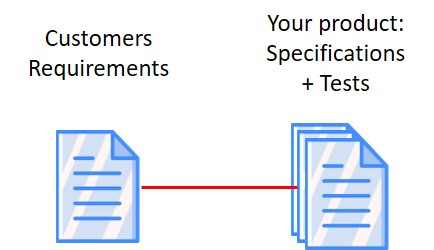
\includegraphics[]{1-in-the-same-document.jpg}
    \caption{The product specifications and tests are in the same document}
    \label{fig:SameDocument}
\end{figure}

Your customer has described his need in a requirements document. You reply to it in a specifications document where you explain all the features of you future product. Each of those features is followed by a corresponding test with a status checkbox telling if it is OK or not.

Like this you reduce the number of documents by gathering everything in one.

But if the project grows and the product requires more complex features, you may want to test several of them at once if you can. This format doesn’t allow this kind of test management: you cannot “factorize” the tests and therefore you may have redundancies. Which is not very efficient.

\subsection{2. List the tests in a separate document}

\begin{figure}[h]
    \centering
    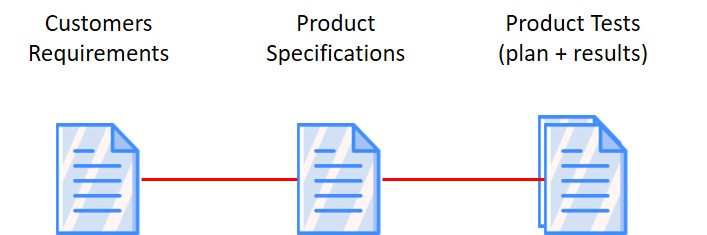
\includegraphics[]{2-in-two-document.jpg}
    \caption{Tests in their own document}
    \label{fig:TwoDocument}
\end{figure}

Your customer has described his needs in a requirements document. You reply to it in a specifications document. And you describe the tests on those specifications in a third document. Each test can have specific fields to precise details on the results (measured values, expected results, status, comments\dots).

The benefit is that you can now factorize the tests: in one bigger test you can check the validity of several specifications at once and reduce the time spent on this activity.

The drawback is now you have to keep track of the links between the specifications and their tests. But it is easy to do so with traceability matrices.

Now, a new hidden problematic comes out. It only occurs if you have to perform your tests several times. Let’s take a concrete example. Imagine you are a reusable anti-COVID masks manufacturer (not the disposable ones). So you deliver lots of masks, all the same, and you have to test each and everyone of them before to put them on the market. For each mask you have to duplicate the test document to perform the campaign, and to fill it with the mask tests results but the test descriptions are exactly the same. That makes a lot of redundancy between the 2 documents. Let’s see how to optimize this…

\subsection{3. Cut the test document in 2: the procedures and the results}

\begin{figure}[h]
    \centering
    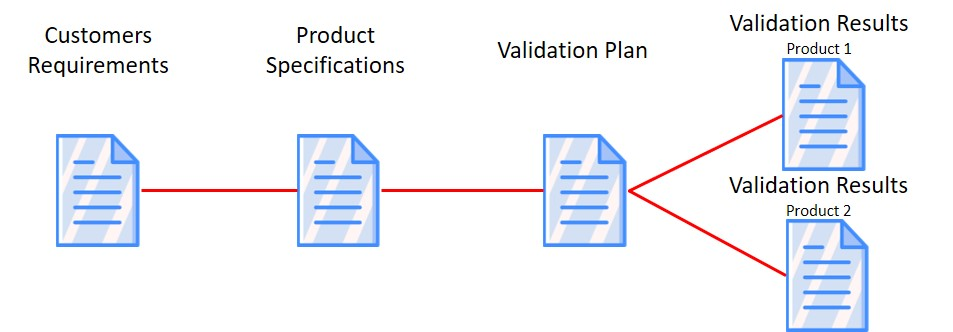
\includegraphics[]{3-in-three-documents.jpg}
    \caption{Test procedures and results in 2 documents}
    \label{fig:ThreeDocument}
\end{figure}

Here is the best way to do, from our point of view:

\begin{itemize}
    \item The tests procedures are detailed in a first document: the validation plan
    \item All the results for the same product are gathered in its own document: the validation results
\end{itemize}

OK the obvious drawback is the multiplication of the documents. From “one doc to rule them all” we go to at least 3 (specifications, validation plan and validation results) and more if you deliver several identical products. And off-course you have to manage a traceability matrix for each document relation (red link).

BUT,

it is the best way for us because of the following reasons:

\begin{itemize}
    \item Each document deals with only one aspect of the project: specifications design the solution, validation plan builds the tests, validation results report the status on the product.
    \item Each document is therefore shorter and so easier to maintain up to date.
    \item Consequently, each document can evolve independently from the other one. And if there is an impact, the traceability matrices will tell you exactly where.
\end{itemize}

In the following sections, we will explain the organizations of the validation plan and results in two separated document. But even if they are merged it works the same.

\section{The procedures}
In the validation plan you will define all the procedures for the required tests to validate that your product correctly matches its specifications.

The validation plan will contain enough tests if and only if all of the specifications are covered by one test at least. Although it doesn’t mean there should be one test for each specification. And this is one major benefit of the validation plan, you can do:

\begin{itemize}
    \item one test for one specification
    \item one test for several specifications at once
    \item several tests to check only one complex specification
\end{itemize}

That’s why traceability matrices are very useful! By tracking all those relations they ensure at least one test covers each specification. If it is not the case, you know you need more tests and what to do them on.

\section{How to structure a test procedure?}
A test procedure is divided in two parts:

\begin{itemize}
    \item The test identification
    \item The test steps
\end{itemize}

\subsection{The test identification}
This identification gathers several metadata about the test itself. Here are the most essential ones.

\subsubsection{A unique reference}
This reference allows to identify instantly the test without any doubt. It will be useful in the traceability matrices. It can be followed by a revision number to track the evolutions on the test: each modification of the text increases its revision number.

Ex.: NPT\_ProjectVehicule\_VP\_0301.1

\subsubsection{A title}
It is required to have a title telling in a few words the purpose of the test. It is essential to quickly know what the test is about, and refer it easily in a conversation with coworkers for example.

Ex.: “Check the front light”

\subsubsection{A description}
You explain here the purpose of the test. What is it doing, why and maybe how the test is supposed to end. Sometimes the person writing the test (the author) is not the same person to perform it (the operator). The description will give the operator some details about the context and what he should expect.

Ex.: “The purpose of this test is to check the front light of the car are correctly working and manageable from the pilot seat.”

\subsubsection{Initial conditions}
This is a very important item! Setting initial conditions allows to sequence your validation plan.

Some tests can require to be done within specific conditions. They may be possible only under certain circumstances.

For example, a test might be so long, it would be easier to cut it in half. Therefore the second part can only be performed if the first part is OK. So the success of part one is the “initial condition” for part two.

Another example, several tests can have their first steps in common. You may want to gather those redundant steps in a dedicated test to do it just once and cut this part from the other tests. You will gain some precious time and those tests require to have this initial condition (the first steps) to be previously done.

Ex.: This test requires the followings tests to be passing:

NPT\_ProjectVehicule\_VP\_0230.1 : Check the car start-up\\
NPT\_ProjectVehicule\_VP\_0254.1 : Check the car’s wiring

\subsubsection{The traceability}
With this item, you list all the specifications this test validates.

So the compilation of all the tests traceabilities tells you exactly which specifications are tested and which are not. So you can calculate the coverage of your validation plan, you know if it is complet or needs some more tests.

Ex.: Coverage:
\begin{itemize}
    \item NPT\_ProjectVehicule\_SPEC\_0058.1
    \item NPT\_ProjectVehicule\_SPEC\_0022.1
    \item NPT\_ProjectVehicule\_SPEC\_0137.1
    \item NPT\_ProjectVehicule\_SPEC\_0796.1
\end{itemize}

\subsubsection{Other possible items}
Here are some items you can add to the test identifications:

\begin{itemize}
    \item \textbf{The kind of test}: tests can be categorized depending on the way to perform them. There are inspection test where you just have to visually check the presence of an element. There are the certification tests where you need to have a certificate from the supplier officially telling you the device is working. The demonstration tests that require to manipulate the device to obtain the expected behavior…
    \item \textbf{The gravity}: some tests may be more important than other. If a low gravity test is not ok, may be it’s not a big deal and the device is still good enough to be delivered. By giving gravity indication on tests, you can sort them to prioritize the most important ones.
\end{itemize}

\subsection{The test steps}
This is here we go deep into the test procedure, step by step. The procedure is basically a table where each line is a test step. I strongly recommend to explicitly sequence the procedure step by step. The best procedure is the one that can be performed by a total stranger to the project as everything is completely detailed.

This exhaustiveness principle brings several benefits:

\begin{enumerate}
    \item Having a crystal clear procedure allows the test operator to focus on the unit under test and how it reacts. But if he has to question the procedure or to guess if he understands it well enough, he will also question the results he observes. He won’t know if he’s doing right or if he misses something if the procedure allows to doubt.
    \item The procedure can be performed by a stranger and this stranger won’t be biased. Such an operator is better at finding bugs or fault (See Fix your product issue with a problem report). Besides if the procedure can be performed by a stranger, and if you need more people to do the tests because of a deadline, anyone can help you!
\end{enumerate}

Let’s see the different columns we suggest you to put in your test procedure:

\subsubsection{Step number}
This number allows precisely identifying the step in a comment, a potential exchange or even in another step to do a loop in the procedure : “If it is NOK, go back to step \#6“.

\subsubsection{Expected result}
This item is not systematic. If the action doesn’t expect a specific one, do not tell one. On the other hand, if there is one and if it will decide the status of the test, therefore you need to be very specific too:

\begin{itemize}
    \item If what is expected is a behavior, then be very detailed about it without any possible doubt. We don’t want the operator to miss it
    \item If a measure is expected: a number of items, a voltage, a length… Then tell the expected measure’s value, unit and tolerance.\\Example: you expect a board to be 2 meters long more or less 1 centimeter (or 0,01 m).\\If the measured length is 2,005 m then the test is OK.
\end{itemize}

\subsubsection{Some other attributes}
Here are some more attributes to add to the procedure table:

\begin{itemize}
    \item \textbf{Traceability} : you can tell for each step the specification it validates. You may just fill it for the steps with an expected result and not for the others. It allows to rapidly see which part of the procedure is critical but it can be redundant with the traceability given in the test identification.
    \item \textbf{How to manage NOK steps}: when a step is OK, we implicitly go for the next one. But what if the step is not OK (NOK)? Should we leave the UUT in this state? You may have to properly shut it down. So you could describe in a new column what to do if the step is NOK. You can write a “shut down procedure” in the validation plan, and you can refer to this procedure in the step in the case where the step is NOK.
\end{itemize}


Et Voilà for the structuring of the test procedures. Don’t forget to add the traceability matrices at the end of the validation plan to keep track of the coverage.

\section{The validation results}
It’s like the little brother of the test procedures. This report document contains all the results of all the tests for one sample of the product to be delivered. And this time, for each procedure there is only one test report. This will ease the traceability matrix between the validation plan and the validation results as their relation is 1:1.

In the previous article, we saw that the benefits of separating the procedures from the results in 2 different documents is to be able to perform the validation plan on several identical products. So the validation results are belonging to one and only one copy of the product. So this is the first thing to do: uniquely identify the copy of the product to be tested.

\subsection{Identifying the UUT}
UUT or Unit Under Test, is the generic name given to the product that is tested. So now I’ll refer to it as the UUT.

In the very beginning of the result document, we will dedicate a paragraph to identify the UUT. The purpose is to associate the result document to only one copy of the product and be sure not to mix it with another copy. Though the serial number is one piece of data to identify a product, here are a list of information useful to complete the identification:

\begin{itemize}
    \item Model number or name. Ex.: “iPhone”
    \item Revision number. Ex.: “12”
    \item Serial number. Ex.: “98765431”
    \item Date of manufacture. Ex.: “October 2020”
\end{itemize}

With all those element : “iPhone 12, S/N: 98765431, October 2020”, we are very sure there is not another copy of the product with the same attributes.
In the eventuality that this precise product is malfunctioning and the customer returns it, it will be easy the find the corresponding validation results to check if all the tests had been correctly done.

To have a better overview, we can define a global validation status telling you at once if the product is OK or not. This status is the compilation of all the test results statuses. This global status can obviously be filled out once all the validation plan tests have been performed at least once. And then, for more details you can go for the procedure result you want.

\subsection{How to structure the results for each procedures?}
Now that the UUT is clearly identified, let’s see the reports. Just like the procedures in the validation plan, they are divided in 2 sections:

\begin{itemize}
    \item The test results identification
    \item The results step by step
\end{itemize}

\subsubsection{The test results identification}

\paragraph{The reference}
Remember, to reduce the size of the report, we decided not to put the procedures in it, so to understand the results we recall the reference of the test procedure they are about.

\paragraph{The title}
For comfort, we repeat the title of the procedure. It easier when you browse the results to look for an understandable title than a cryptic reference.

(So now you think: what’s the purpose of the reference then? Well, when you need to refer to the test in another document, you will prefer a short reference to a long explicit title.)

\paragraph{The timestamp}
We tell the date and time of the moment the results has been obtained / the test sequence has been performed. This would be very useful in case of a future issue with this product. We will be able to cross those data with some other data, like log files or automatic reports from other tools, if we need to investigate.

\paragraph{Identification of the test operator}
When several people have to perform the tests or when the operator is different from the developer, it is useful to identify them.

In case of a failed test, the person in charge of fixing the problem may need some more information and would question the operator (See Problem Report, Fix your product issue).

\paragraph{The test status}
This is the most important piece of information. It is the compilation of all the step statuses. It can tell in a glimpse if the UUT has passed the procedure or not. If not, we can go look for the test comments or for the specific failed step.

Commonly, for a test to be fully “OK”, all the steps must be successfully passed.
On the other side, for the test to fail, it only requires one step to be not OK!

But a failed test doesn’t necessarily imply the UUT is deficient. Maybe the procedure isn’t mature enough and needs to be updated.

\paragraph{Comment}
It allows the operator to add some precision elements about the course of the procedure. He can write down observations and details about what happened when the test failed for example.

\paragraph{Those attributes we do not repeat from the procedure}
As the relation between the report and the procedure are 1:1, there is no need to repeat the test description, the traceability or the initial conditions. They would only make the report heavier and its update more difficult (that’s why we cut it in half).

\subsubsection{The results step by step}
\paragraph{Step number}
This is the same number we have on the procedure to link the result to the corresponding step.

\paragraph{Measure}
This column allows to enter a measure eventually required by the step. If the step doesn’t ask for it, leave a blank case.

\paragraph{Status}
You can set a status for each step telling if it has been passed successfully or not:

\begin{itemize}
    \item \textbf{Done} / \textbf{OK}: for a step that doesn’t expect any specific result. Therefore you simply check it was done, so a checkbox could be enough.
    \item \textbf{OK}: the step required a specific result that perfectly happened.
    \item \textbf{NOK} (for Not OK) / \textbf{Failed} : the step required a specific result that didn’t happen as expected.
\end{itemize}

\paragraph{Step comment}
Having a comment column to add details to a specific test in case of a failure can be really helpful to investigate the problem.

\paragraph{Some other possible attributes}
\textbf{Action}: When a step fails, it might be because of an issue with the UUT and a problem report should be initiated. Or it may be because of the test procedure that must be updated, in this case a reading sheet shall gather the remarks about the procedure. Therefore the Action field is used to give the reference of such file that will document the fixing action. So you can track all the strategy and all the modifications upon the procedure.

This concludes our proposition for a better structure of the product validation plan. Now I’d like to draw your attention on one last thing to reach a greater quality level.

\section{The importance for the author, the maker and the test operator to be 3 different people}
This measure can look expensive at first, but if you have to perform tests at great scale, it can significantly reduce the bias and increase the quality.

First of all, the author is the collaborator writing the tests procedures. This is the person who has designed them.
The maker is the person who has built the product or realized the service. He has shaped what was designed.
And finally the test operator is the one performing the tests (designed by the author) onto the product (built by the maker).

In a perfect world (and such a world is very expensive, we all agree), all three of them are different people. But in practice, because of the budget or the planning, all of them might be merged into the same person. This person knows perfectly its product. So when she tests it, she can unconsciously but slightly adapt the procedure to make it pass. Or worse, she will be willing to make it pass. But this is precisely the point of the test: finding the failures to fix them before delivery.
In the other way, a different person as the test operator will have no idea on how a product works. So he will methodically follow the procedure and be very good at finding those failures (from the product or from the procedure).

That is why it is very efficient to separate those 3 steps in the development of a product : design, realization and tests. It will reduce the risks of human bias or conflict of interest. But they need to work very closely to avoid inertia. A project management is always a clever compromise between quality, cost and delays.

(In the end, it is one more reason for identifying the person performing the test in the report!)

\section{Conclusion}
As we saw it in this article, building and performing a test plan is a real project within a project. But it is essential to ensure a high quality product.

It would be easy to believe that the multiple documents, detailed here, make the project management heavier. But at the end of the day, they don’t. Yes they require a little more time at the beginning of the project but they induce more flexibility and therefore a better resilience. Ok there are more documents but they are shorter and easier to maintain.

If the customer’s requirements evolve, you’ll only have surgical modifications to make which will be pointed out by the traceability matrices.

% \input{chapters/organize_documents.tex}
% \input{chapters/svn.tex}
% \input{chapters/write_specifications.tex}
% \input{chapters/review.tex}
% https://www.naept.com/blog/compliance-matrix-how-to-manage-a-request-for-proposal/
\setchapterpreamble[u]{\margintoc}
\chapter{Compliance Matrix\\A tool to break a request for proposal}
\label{sec:ComplianceMatrrix}

You have just received a new request for proposal from a customer. A big one. 30 pages, several expertise domains required, almost a hundred requirement. You have to sort it out. You will need a compliance matrix!

\section{The purpose}
Sometimes the RFQ are rather light and request a short proposal. But, if on the contrary, the request is very detailed then its treatment requires a deep study to :

\begin{itemize}
    \item understand well-enough what is asked
    \item precisely explain your solution
\end{itemize}

Besides you may face some competitors on the market so you cannot loose any time. Therefore you have to be fast and organized. The compliance matrix is a tool allowing you to manage every components of your customer need to define what to do with it : ask for more information, go for it, subcontract…

So basically a compliance matrix is a kind of conversion box that takes the customer’s request as an input and produces your treatment for its need, aka your solution as an output.

\section{The format}
Just like the reading sheet, the compliance matrix is a simple spreadsheet document. So you can build one from your favorite editor. You can download for free a model we made after multiple customer feedbacks. This is a Microsoft Excel template format. Which means every time you double click on it, it creates a copy of the original file. If you want to modify the template to add your own reusable content, just right click on it and hit modify.

\section{The content}

Let’s see what the headers of this matrix are and how to fill this table.

Each line of the matrix represents the management of a specific need expressed by the customer. We call such a need assessment: a requirement. The blue columns contain the data issued from the customer, and the yellow ones are about your way to manage them.

And last disclaimer, such a matrix is highly versatile. Each company has its own version. The columns vary a lot depending on your RFQ treatment workflow, the size of your company, the number of people involved in the process, the complexity of the customer’s need, … We have encountered dozens of different kind of matrices. Here we present the most common headers and the management they induce. So feel free to download our template and update it to your needs.

\begin{table*}[h]
	\centering
		\begin{tabular}{|c|c|c|c|c|c|c|c|c|c|}
			\hline
			ID & Source & Location & Reference & Content & Theme & MoSCoW & Impacts & Risk & Management & Analysis Comment & Go or NoGo \\ 
			\hline
			&&&&&&&&&\\
		\end{tabular}
	\caption{Headers for a reading sheet}
	\label{tab:HeaderRS}
\end{table*}

\subsubsection{ID}
This is just the number of the line. It helps communicating on the matrix with the other people on the project. By default, as soon as you deal with an array of any kind, it is a good practice to give a simple iterative id to the lines in order to keep track of the new entries.

\subsubsection{Source}
This is the document title / name where the customer requirement comes from.

Sometimes the customer RFQ is a unique document, so every requirement will have the same Source. But it can happen that its need is described in multiple documents like in the construction industry where you have a main file explaining the global project and many annexes detailing specific aspects.

\subsubsection{Location}
The document can be hundred of pages long, so it might be useful to indicate where in the document this requirement is located. This is the purpose of this column.

We recommend to not indicate a page number because they might evolve from a document revision to another. Instead we suggest to give the title or the number of the smallest sub-section containing the requirement.

\subsubsection{Reference}
Here you identify precisely the requirement. You can either put the reference if there is one, or a simple title. The purpose here is to know what requirement we are talking about.

\subsubsection{Content}
This item is optional but as it is very frequently displayed in compliance matrices we encountered, we did put it in our template.

If the requirement is relatively short, you can copy it here. It avoids having to look for it in the document. It eases the management but what if the requirement evolves ? You will have to remember to update it. So you must be careful with this item. The most important is to fill the 3 previous ones (source, location and requirement reference) to ensure the traceability.

\subsubsection{Theme}
Here you tell, in one or two words, what the requirement is about, what expertise is involved or what kind of technology. For example : legals, mechanics, web development, marketing, …

The purpose of this item is to sort, classify, categorize the requirement to ease its management. So if an expert in mechanics has to have a quick look, he can filter the content by his field of expertise.

\subsubsection{MoSCoW}
This one is very interesting. It is about the MoSCoW method which allows to prioritize the requests. It tells the criticality level of a need. MoSCoW is an imperfect acronym to memorize in order the different levels :

\begin{itemize}
    \item M for Must. An M requirement is an absolute need for the customer
    \item S for Should.
    \item C for Could.
    \item W for Wish. Sometimes it says W for Won’t.
\end{itemize}

This scale is very personal for every one. So if your customer gives you its signification or another classification, this is a very precious element telling you where are the pain point.

If he doesn’t give you such information, it could be very interesting to ask him for it. Or maybe it means that every requirement is equally needed. It’s worth asking.

\subsubsection{Impacts}
Here we enter the columns that are specific to your own management. So starting with this one until the last, you may want to adapt them.

Impacts is a collection of several columns : Field 1, Field 2, … Those fields should be replaced by your different departments / services / expertise domains. Then complete the column by putting an “X” or a “1” (we prefer 1 so you can apply formula more easily) when a requirement is impacting one of your fields.

When the requirement is complex, it might involve several expertise domains and those columns are another way to classify the requirement. For example, you could have a project manager who initiates the compliance matrix. He reads the RFQ, identify the requirement in the table and for each of them he sets 1 where they must be reviewed by this or that expert. So when the expert received the matrix, he sorts the requirement by his own field so he doesn’t have to read all the RQF.

\subsubsection{Risk}
To every requirement, it is possible to give a risk level : whether it is totally safe to do or we anticipate future difficulties on this requirement.

Here too, the way to evaluate risk is very specific to a company. So, in our template, we just put a scale from 1 to 5. Feel free to define 1 or 5 as your maximum risk level or even to define another scale.

\subsubsection{Management}
This new set of columns represents your way to deal with the requirement during the analysis. We suggest in our template 4 possible managements for requirement :

\begin{itemize}
    \item Technical Analysis : the requirement is complex and requires one of your specialists to have a look and give his opinion.
    \item Customer clarification : the requirement is not very clear and you have some questions about it for your customer. Once the requirement is clarified, a new management decision shall be made.
    \item Internal execution : the requirement is clear, your company has the skills to deal with it. It is a green light.
    \item Subcontracting : the requirement is understood, your company cannot execute it but you have a supplier you can subcontract it to.
\end{itemize}

Those 4 ways may not cover all the possibilities, they are just examples. Complete them with your own internal processes.

\subsubsection{Analysis / Comment}
This section is to give some details about either the expert analysis or just the requirement itself. It shall be used by any contributors to give enlightenment or ask questions about the management or the understanding of the requirement.

\subsubsection{Go / NoGo}
And finally, once the requirement understanding and management has been fully processed, you can tell here if it is a Go or a NoGo. In other words, you say Go when you can deal with the requirement whatever the management you chose, and you say NoGo when you cannot or you prefer not to because it is too risky.

\section{Conclusion}
Of course the best case scenario is to Go on all requirements, but identifying very early in the process the risks or the impossibilities on a project is the power of the compliance matrix. It is better to find them out at the beginning than several months into the project. At that stage the cost of fixing them could be multiplied several times and put at risk not only your company but your customer’s too!

The compliance matrix is another very powerful tool allowing you to cut a big request in lots of smaller simpler ones. Even if you customer has written a big continuous and not well structured need description, you can use the matrix to cut it, identify requirements within it and manage them all flawlessly.
% \input{chapters/rfq_analysis.tex}
% \input{chapters/rfq_building.tex}
% \input{chapters/rfq_content.tex}

%----------------------------------------------------------------------------------------

\backmatter % Denotes the end of the main document content
\setchapterstyle{plain} % Output plain chapters from this point onwards

\end{document}
